\documentclass[11pt,letterpaper]{article}
\usepackage[margin=1in,headheight=14pt,headsep=8mm]{geometry}
\usepackage{fontspec}
\IfFontExistsTF{Liberation Serif}{%
  \setmainfont{Liberation Serif}%
}{%
  \setmainfont{Times New Roman}%
}
\IfFontExistsTF{Liberation Sans}{%
  \setsansfont{Liberation Sans}%
}{%
  \IfFontExistsTF{Latin Modern Sans}{%
    \setsansfont{Latin Modern Sans}%
  }{%
    \setsansfont{Helvetica}%
  }%
}
\IfFontExistsTF{DejaVu Sans Mono}{%
  \setmonofont[Scale=0.84]{DejaVu Sans Mono}%
}{%
  \IfFontExistsTF{Menlo}{%
    \setmonofont[Scale=0.82]{Menlo}%
  }{%
    \setmonofont[Scale=0.84]{Courier New}%
  }%
}
\usepackage{amsmath,amssymb,amsthm}
\usepackage{microtype}
\usepackage{setspace}
\setstretch{1.18}
\usepackage{longtable,booktabs,array,calc}
\newcounter{none}
\usepackage{needspace}
\usepackage{graphicx}
\usepackage{fancyhdr}
\usepackage[authoryear,round]{natbib}
\usepackage{xcolor}
\definecolor{linkblue}{HTML}{1B365D}
\PassOptionsToPackage{hyphens}{url}
\usepackage[unicode,colorlinks=true,allcolors=linkblue,bookmarksnumbered=true]{hyperref}
\usepackage{xurl}
\urlstyle{same}
\hypersetup{pdftitle={What Prediction Leaves Out: Relational Objecthood
and the Grounds of
Purpose},pdfauthor={},pdfsubject={Philosophy of Science Double-Anonymous Submission}}
\setlength{\parindent}{1.15em}
\setlength{\parskip}{2pt}
\setlength{\emergencystretch}{2.5em}
\setcounter{secnumdepth}{2}
\widowpenalty=10000
\clubpenalty=10000
\providecommand{\tightlist}{\setlength{\itemsep}{2pt}\setlength{\parskip}{0pt}}
\providecommand{\passthrough}[1]{#1}
\pagestyle{fancy}
\fancyhf{}
\fancyhead[L]{\footnotesize What Prediction Leaves Out}
\fancyhead[R]{\footnotesize \emph{Philosophy of Science} (Anonymous Submission)}
\fancyfoot[C]{\small\thepage}
\renewcommand{\headrulewidth}{0.25pt}
\fancypagestyle{plain}{\fancyhf{}\fancyfoot[C]{\small\thepage}\renewcommand{\headrulewidth}{0pt}}
\begin{document}
\thispagestyle{plain}
\begin{center}
{\fontsize{17.5}{22}\selectfont\bfseries What Prediction Leaves Out:
Relational Objecthood and the Grounds of Purpose\par}
\end{center}
\vspace{4pt}
\begin{abstract}
\noindent When does predictive adequacy warrant ontological claims about
persistence or teleological claims about purpose? For four founders
executing hereditary programs autonomously at fixed parameters in a
stochastic repair-and-reproduction model, undamaged and repaired
conservative founders share the exact infinite-horizon birth law while
paying zero versus three repair units. Two birth censuses saturate
infinite-horizon birth laws, separating latent programs while erasing
repair cost; adjoining initial cost separates repair histories while
merging damaged programs, yielding incomparable law refinements (though
single runs overlap). Proliferation can maximize lineage growth while
lowering parent survival, motivating calibrated relational objecthood
and bearer-indexed purpose.
\end{abstract}
\vspace{8pt}

\section{Introduction: The explanatory transfer
problem}\label{introduction-the-explanatory-transfer-problem}

Consider an engineered or biological device whose damaged active
instruction register is restored by majority vote from surviving
internal copies before generating its next output, alongside an
undamaged twin. Once restoration completes, both induce the \emph{exact
same probability law} over the entire infinite sequence of subsequent
births: neither larger samples nor longer horizons distinguish undamaged
operation from paid restoration. Across four founders executing
conservative or proliferative hereditary programs autonomously at fixed
parameters, adding a second birth census already saturates
infinite-horizon birth laws---separating latent programs while erasing
three-unit repair expenditure---whereas adjoining first-step metabolic
cost separates paid from unpaid histories while leaving damaged programs
merged. Different protocol expansions thus produce \emph{mutually
incomparable refinements} over probability laws, establishing a sharper
thesis than the truism that prediction differs from explanation:
\emph{which class of evidence is added determines which explanatory
question becomes identifiable}. Finally, switching from conservative
maintenance to proliferation can raise expected descendants per cycle
while lowering parent survival, leaving ``adaptive for persistence''
ambiguous until its bearer---parent token, re-instantiated organization,
or lineage---is specified.

These cases exemplify the \emph{explanatory transfer problem}. Across
science and philosophy, predictive compression and optimization are
widely treated as guides to ontology and teleology: pattern realism ties
objecthood to non-redundant compression
\citep{dennett1987, dennett1991, ladymanRoss2007, wimsatt2007};
computational mechanics and predictive state representations define
minimal states from future laws
\citep{crutchfieldYoung1989, shaliziCrutchfield2001, littmanSuttonSingh2001, barnettCrutchfield2015};
active inference moves from Markov blankets to autonomous agency
\citep{friston2010, friston2013, clark2013, parrPezzuloFriston2022}; and
inverse reinforcement learning fits scalar rewards to behavior
\citep{puterman1994, ngRussell2000}.

Selective representation is indispensable; trouble begins when
predictive adequacy on one channel is transferred to claims about
mechanism, persistence, or purpose whose truth conditions depend on
distinctions quotiented away. Recent critiques of blanket metaphysics
\citep{raja2021, bruineberg2022} and organizational normativity
\citep{corti2023, bich2024, cuciniello2026} expose parts of this gap,
yet lack a unified formal diagnosis of cross-protocol
non-identifiability paired with constructive compatibility conditions.

Underlying our results is a \emph{forward-marginalization asymmetry}:
predictive sufficiency marginalizes over past pathways to retain
equivalence classes of forward output laws, erasing counterfactual
invariance, paid repair, and genealogy. Governed by a typed
\emph{principle of explanatory preservation}, we defend three theses
(proofs in Appendix A):

\begin{enumerate}
\def\labelenumi{\arabic{enumi}.}
\tightlist
\item
  \textbf{Constrained relational objecthood.} Three exclusionary
  criteria---\emph{(i) predictive--control compression}, \emph{(ii)
  counterfactual intervention invariance}
  \citep{hacking1983, woodward2003, craver2007}, and \emph{(iii)
  realization-cost accountability}
  \citep{jonas1966, rosen1991, montevilMossio2015}---eliminate passive
  blankets and cost-free shadows while leaving symmetrical fission
  conventions explicit.
\item
  \textbf{Bearer-indexed grounds of purpose.} Purposive claims are
  indexed to bearer, contrast class, mechanism, and ground across four
  levels: \emph{(Rung 1) systemic role} \citep{cummins1975}, \emph{(Rung
  2) conditional regulatory and repair standards}
  \citep{rosenblueth1943, mossio2009, diPaolo2005, bich2024},
  \emph{(Rung 3) retrospective selective retention or reproduction}
  \citep{wright1973, millikan1984, godfreySmith1994, garson2019}---separated
  from prospective growth---and \emph{(Rung 4) practical reason}
  \citep{korsgaard1996, scanlon1998, street2006}.
\item
  \textbf{Benchmarking autonomous programs against full-policy
  ceilings.} Within a unified regenerative model \(\mathcal{M}\), we
  benchmark \emph{autonomous hereditary execution} against the
  \emph{full public-history growth ceiling}
  \(\rho_* = \max\{1, \lambda_0, \lambda_1\}\), separating hereditary
  persistence from dormancy switching.
\end{enumerate}

Section 2 establishes predictive minimality, belief-quotient descent,
and relational objecthood; Section 3 constructs \(\mathcal{M}\) and
proves incomparable refinements and gate separation; Section 4 analyzes
paid repair, finite-memory viability, and fission; Section 5 proves
evaluative underdetermination, Theorem 1, and four-rung purpose; Section
6 addresses rival programs, objections, and tests; Section 7 concludes.

\section{Predictive equivalence, sufficient quotients, and relational
objecthood}\label{predictive-equivalence-sufficient-quotients-and-relational-objecthood}

\subsection{Protocol-indexed predictive minimality and its
limits}\label{protocol-indexed-predictive-minimality-and-its-limits}

Let \((\mathcal{H}, \Sigma_{\mathcal{H}}, \mu)\) be a probability space
of realized histories up to a decision point, and let \(\mathcal{I}\) be
a countable index set of observation or open-loop test protocols, each
assigning to \(h \in \mathcal{H}\) a Markov response kernel
\(K_i(h, \cdot)\) on a countably generated space
\((\mathcal{Y}_i, \Sigma_{\mathcal{Y}_i})\)
\citep{blackwell1953, kallenberg2021}. The \emph{canonical predictive
representation} for \(\mathcal{P} = \{K_i\}_{i \in \mathcal{I}}\) is
\(C_{\mathcal{P}}(h) := (K_i(h, \cdot))_{i \in \mathcal{I}}\), inducing
\(h \sim_{\mathcal{P}} h' \iff C_{\mathcal{P}}(h) = C_{\mathcal{P}}(h')\).

\textbf{Proposition 1 (Countable-protocol predictive minimality).}
\emph{Suppose \(\mathcal{I}\) is countable and each
\((\mathcal{Y}_i, \Sigma_{\mathcal{Y}_i})\) is countably generated. If
\(q: (\mathcal{H}, \Sigma_{\mathcal{H}}) \to (\mathcal{Z}, \Sigma_{\mathcal{Z}})\)
is predictively sufficient for \(\mathcal{P}\) on
\((\mathcal{H}, \Sigma_{\mathcal{H}}, \mu)\)---so for every
\(i \in \mathcal{I}\) there exists a measurable kernel
\(\widetilde{K}_i\) with
\(K_i(h, \cdot) = \widetilde{K}_i(q(h), \cdot)\) \(\mu\)-almost
everywhere---then there exists a measurable decoder
\(\psi: \mathcal{Z} \to \prod_{i \in \mathcal{I}} \Delta(\mathcal{Y}_i)\)
such that \(C_{\mathcal{P}}(h) = \psi(q(h))\) for \(\mu\)-almost every
\(h \in \mathcal{H}\).}

Proposition 1 generalizes causal-state minimality
\citep{crutchfieldYoung1989, shaliziCrutchfield2001}, predictive state
representations \citep{littmanSuttonSingh2001}, and
\(\varepsilon\)-transducers \citep{barnettCrutchfield2015}.
Computational mechanics thus indexes minimality to a chosen process,
subject to three transfer boundaries: countability of \(\mathcal{I}\)
and standard Borel spaces underwrite almost-everywhere factorization and
recursive filtering \citep{astrom1965, kaelbling1998}; passive input
conditioning matches \(\mathrm{do}(A=a)\) only under non-confounding,
non-anticipatory action semantics \citep{pearl2009, woodward2003}; and
\emph{predictive classes are response types, not enduring tokens}
\citep{wiggins2001}.

\subsection{Typed explanatory preservation and quotient
descent}\label{typed-explanatory-preservation-and-quotient-descent}

Exact attribution of \(F: \mathcal{S} \to \mathcal{V}\) from
\(q: \mathcal{S} \to \mathcal{Z}\) requires \(F = \bar{F} \circ q\)
(fiber-constancy). Our \emph{Typed Principle of Explanatory
Preservation} requires specifying
\(\langle \mathcal{B},\, F,\, \mathcal{M}_{\mathrm{prec}},\, \mathcal{I}\rangle\)---bearer,
invariant, precision mode, and interventions---across four tiers:
\emph{(1) token-level attribution}, requiring fiber-constancy on
\((q(h), E_{\mathrm{aux}}(h))\); \emph{(2) distributional attribution},
where a justified fiber prior \((1/2, 1/2)\) over costs \(\{0,3\}\)
preserves mean cost \(3/2\) without identifying individual histories;
\emph{(3) closed-loop belief descent}
\citep{burkeRosenblatt1958, kemenySnell1960, poupartBoutilier2003, givanDeanGreig2003};
and \emph{(4) counterfactual transport} across every interventional
kernel \(P^{\mathrm{do}(\iota)}\) (\(\iota \in \mathcal{I}\))
\citep{woodward2000, rubenstein2017}.

\textbf{Proposition 2 (Exact belief-quotient descent via closed test
spaces).} \emph{Let \((\mathcal{X}, \mathcal{A}, \mathcal{O}, T, O)\) be
a finite partially observed Markov control model, and let
\(\mathcal{F} \subseteq \mathbb{R}^{\mathcal{X}}\) be a linear subspace
with \(\mathbf{1} \in \mathcal{F}\) inducing
\(b \equiv_{\mathcal{F}} b' \iff \forall f \in \mathcal{F},\ \langle b, f\rangle = \langle b', f\rangle\).
Define
\((U_{a,o} f)(x) := \sum_{x'} T(x' \mid x, a) O(o \mid a, x') f(x')\).
Then \(\Delta(\mathcal{X})/{\equiv_{\mathcal{F}}}\) jointly preserves
(i) one-step observation probabilities \(p(o \mid b, a)\) and (ii)
normalized posterior equivalence
\(\mathrm{Bayes}(b,a,o) \equiv_{\mathcal{F}} \mathrm{Bayes}(b',a,o)\)
across all positive-probability branches \((a,o)\) if and only if
\(U_{a,o}\mathcal{F} \subseteq \mathcal{F}\) for all \((a,o)\).}

Sufficiency in Proposition 2 holds on any
\(\equiv_{\mathcal{F}}\)-saturated belief set, whereas necessity uses
interior perturbations on \(\Delta(\mathcal{X})\) (on a forward-closed
reachable set \(\mathcal{R}\), exact recursion requires matching
observation laws and posterior \(\mathcal{F}\)-expectations only on
reachable pairs in the same \(\equiv_{\mathcal{F}}\)-fiber, not
invariance on \(\operatorname{span}(\mathcal{R})\)). Crucially,
\(U_{a,o}\mathcal{F} \subseteq \mathcal{F}\) preserves neither sunk
repair costs nor surgical interventions without expenditure tracking
(Tier 1) and \(\mathrm{do}(\iota)\)-consistency (Tier 4).

\subsection{Against pure compressionism and blanket
metaphysics}\label{against-pure-compressionism-and-blanket-metaphysics}

Constructive empiricists restrict warrant to observable adequacy
\citep{vanFraassen1980}, whereas structural realists defend relations
preserved across theory change \citep{worrall1989, ladyman1998}.
Dennett's \citeyearpar{dennett1991} \emph{Real Patterns} and Ladyman and
Ross's \citeyearpar{ladymanRoss2007} \emph{Rainforest Realism} ground
objecthood in projectible compression, while free-energy theorists treat
stationary \emph{Markov blankets} as individuating self-evidencing
agents \citep{friston2013, parrPezzuloFriston2022}.

While rightly rejecting Lockean essences
\citep{whitehead1929, dupre1993, dupreNicholson2018}, passive output
compression underdetermines causal persistence: epistemic \emph{Pearl
blankets} arise in passive diffusions and Gaussian slices lacking
cohesion \citep{raja2021, bruineberg2022, biehl2021}, and minimal output
compression erases paid repair (Proposition 3). Liberalized pattern
realism can accommodate this by adding interventional and calorimetric
channels; our advance specifies \emph{which added channel licenses which
claim}. \emph{Constrained Relational Objecthood} requires \emph{(1)
multi-channel predictive--control compression} \citep{wimsatt2007},
\emph{(2) counterfactual intervention invariance}
\citep{hacking1983, woodward2003, craver2007}, and \emph{(3)
realization-cost accountability}
\citep{jonas1966, rosen1991, montevilMossio2015}, excluding passive
output shadows \citep{cartwright1999} while leaving symmetrical fission
(Section 4.3) explicit.

\section{A unified stochastic regenerative model of repair, execution,
and
reproduction}\label{a-unified-stochastic-regenerative-model-of-repair-execution-and-reproduction}

\subsection{Physical architecture, internal programs, and resource
accounting}\label{physical-architecture-internal-programs-and-resource-accounting}

We construct a finite stochastic regenerative process \(\mathcal{M}\)
(Table 1; Figure 1a; Appendix A.3). At census \(t \in \mathbb{N}\), each
living token possesses: \emph{(i) two three-bit instruction rows}
\((r_H, r_D)\)---one \emph{active cell} and two \emph{backup cells} per
row---encoding conservative \texttt{care} (\(0\)) or proliferative
\texttt{bloom} (\(1\)); \emph{(ii) a physical execution gate}
\(g \in \{\mathrm{open}, \mathrm{closed}\}\) required for raw actuation;
\emph{(iii) a bootstrap majority-vote unit}
\(b_{\mathrm{boot}} \in \{0,1\}\); \emph{(iv) a six-unit per-step
budget} (\(1\) carried escrow unit plus \(5\) local inflow units: repair
costs \(3\), \texttt{care} costs \(1\), \texttt{bloom} costs \(2\), and
\(2\) units escrow up to two outputs); and \emph{(v) genealogical
identity} (parental retention vs.~strict birth) plus a causally silent
physical tag \(\tau\).

Compare hereditary programs
\(\theta_0 = (\mathrm{care}, \mathrm{care})\) and
\(\theta_1 = (\mathrm{bloom}, \mathrm{care})\). Standard damage flips
both active bits while preserving backups and \(b_{\mathrm{boot}}=1\),
closing \(g = \mathrm{closed}\); internal gate/parity diagnosis
\(d \in \{H, D\}\) is exposed on the public interface read by
\(\Pi_{\mathrm{pub}}\). Damaged \texttt{care} spends \(3\) units on
majority restoration, reopens \(g\), and spends \(1+2=3\) on
\texttt{care} (\(6\) total). Damaged \texttt{bloom} requires
\(3+2+2=7 > 6\): hardware \emph{rejects} it, refunds inflow, and retains
the damaged token w.p. \(1\). Executed steps copy restored rows before
post-step damage hits each output independently w.p. \(q\);
\texttt{stop} terminates with zero outputs.

\Needspace{24\baselineskip}

{\def\LTcaptype{none} % do not increment counter
\begin{longtable}[]{@{}
  >{\raggedright\arraybackslash}p{(\linewidth - 4\tabcolsep) * \real{0.3333}}
  >{\raggedright\arraybackslash}p{(\linewidth - 4\tabcolsep) * \real{0.3333}}
  >{\raggedright\arraybackslash}p{(\linewidth - 4\tabcolsep) * \real{0.3333}}@{}}
\toprule\noalign{}
\begin{minipage}[b]{\linewidth}\raggedright
Component or Transition
\end{minipage} & \begin{minipage}[b]{\linewidth}\raggedright
Formal Specification in Process \(\mathcal{M}\)
\end{minipage} & \begin{minipage}[b]{\linewidth}\raggedright
Resource \& Causal Constraint
\end{minipage} \\
\midrule\noalign{}
\endhead
\bottomrule\noalign{}
\endlastfoot
Healthy \texttt{care} (\(H, \mathrm{care}\)) & Retains parent w.p.
\(s\); 1 strict newborn w.p. \(b\) & Repair \(0 +\) action \(1 +\)
escrow \(2 \le 6\) \\
Healthy \texttt{bloom} (\(H, \mathrm{bloom}\)) & Retains parent w.p.
\(s - \delta\); 1 strict newborn w.p. \(b + \gamma\) & Repair \(0 +\)
action \(2 +\) escrow \(2 \le 6\) \\
Damaged repaired \texttt{care} (\(D, \mathrm{care}\)) &
Majority-restores active bits, opens \(g\), runs \texttt{care}
(\(s, b\)) & Repair \(3 +\) action \(1 +\) escrow \(2 = 6\) \\
Damaged \texttt{bloom} (\(D, \mathrm{bloom}\)) & Prepayment \(7 > 6\):
rejected; damaged token kept w.p. \(1\) & No repair, inflow refunded,
\(0\) births \\
Output inheritance \& damage & Outputs copy restored rows; active bits
damaged w.p. \(q\) & \(H\) at \(t+1\) w.p. \(1-q\); \(D\) w.p. \(q\) \\
\end{longtable}
}

Table 1. Architecture, strict parameters (\(0 < \delta < s < 1\),
\(b,\gamma > 0\), \(b+\gamma < 1\), \(0 < q < 1\)), and six-unit budget
of \(\mathcal{M}\).

\subsection{Task-relative predictive partitions and incomparable
refinements}\label{task-relative-predictive-partitions-and-incomparable-refinements}

On the four single-founder configurations
\(\{\theta_0 H, \theta_0 D, \theta_1 H, \theta_1 D\}\) executing
hereditary programs autonomously at any fixed strict parameter vector in
Table 1 (independent of demographic growth regimes), let \(B_t\) count
strict births at census \(t\) and \(R_1 \in \{0,3\}\) denote initial
repair expenditure.

\textbf{Proposition 3 (Two--three--four predictive separation, two-step
saturation, and incomparable refinements).} \emph{Under autonomous
hereditary execution in \(\mathcal{M}\) at any fixed strict parameter
vector in Table 1: (1) predicting \(B_1\) yields \textbf{two} minimal
law classes, \(\{\theta_0 H, \theta_0 D, \theta_1 D\}\) and
\(\{\theta_1 H\}\); (2) predicting \((B_1, B_2)\) already saturates all
finite birth records \((B_1,\dots,B_T)\) (\(\forall T \ge 1\), hence
\((B_t)_{t\ge 1}\)), refining \((B_1)\) to \textbf{three} classes,
\(\{\theta_0 H, \theta_0 D\}\), \(\{\theta_1 D\}\), and
\(\{\theta_1 H\}\), coupling \(\theta_0 H\) and \(\theta_0 D\)
identically for all \(t \ge 1\) while separating \(\theta_0 D\) from
\(\theta_1 D\) at \(t=2\)
(\(\mathbb{E}_{\theta_1 D}[B_2] - \mathbb{E}_{\theta_0 D}[B_2] = (s+b)(1-q)\gamma > 0\);
\(27/64\) vs.~\(39/64\) at \((3/4,1/8,3/8,1/4,1/3)\)); (3) predicting
\((B_1, R_1)\) refines \((B_1)\) to an incomparable \textbf{three}-class
partition
\(\{\theta_0 H\}, \{\theta_1 H\}, \{\theta_0 D, \theta_1 D\}\), while
\((B_1, B_2, R_1)\) yields \textbf{four} singleton law classes.}

\Needspace{24\baselineskip}

{\def\LTcaptype{none} % do not increment counter
\begin{longtable}[]{@{}
  >{\raggedright\arraybackslash}p{(\linewidth - 4\tabcolsep) * \real{0.3333}}
  >{\raggedright\arraybackslash}p{(\linewidth - 4\tabcolsep) * \real{0.3333}}
  >{\raggedright\arraybackslash}p{(\linewidth - 4\tabcolsep) * \real{0.3333}}@{}}
\toprule\noalign{}
\begin{minipage}[b]{\linewidth}\raggedright
Observation Protocol \(\mathcal{P}\)
\end{minipage} & \begin{minipage}[b]{\linewidth}\raggedright
Minimal Classes of Protocol Laws on
\(\{\theta_0 H, \theta_0 D, \theta_1 H, \theta_1 D\}\)
\end{minipage} & \begin{minipage}[b]{\linewidth}\raggedright
Unidentifiable from Protocol Law
\end{minipage} \\
\midrule\noalign{}
\endhead
\bottomrule\noalign{}
\endlastfoot
One-step strict births \((B_1)\) &
\(\{\theta_0 H, \theta_0 D, \theta_1 D\}\), \(\{\theta_1 H\}\) (2 law
classes) & Latent \(\theta_1\) in \(\theta_1 D\) \& repair fee
\(R_1\) \\
Births \((B_1, B_2) \equiv (B_t)_{t\ge 1}\) &
\(\{\theta_0 H, \theta_0 D\}\), \(\{\theta_1 D\}\), \(\{\theta_1 H\}\)
(3 law classes) & Founder repair expenditure \(R_1 \in \{0,3\}\) \\
One-step births + fee \((B_1, R_1)\) & \(\{\theta_0 H\}\),
\(\{\theta_1 H\}\), \(\{\theta_0 D, \theta_1 D\}\) (3 law classes) &
Hereditary difference \(\theta_0 D\) vs.~\(\theta_1 D\) \\
Two-step births + fee \((B_1, B_2, R_1)\) & Four singleton law classes
(4 distinct laws) & Silent tag \(\tau\) (single runs still overlap) \\
\end{longtable}
}

Table 2. Diamond lattice of minimal predictive partitions over protocol
laws in \(\mathcal{M}\) at fixed parameters, showing two-step birth
saturation and two incomparable three-class refinements.

At fixed parameters, two censuses \((B_1, B_2)\) exhaust
\((B_t)_{t\ge 1}\) across these four autonomous founders: post-step
confluence and escrow clearing merge \(\theta_0 H\) (\(R_1=0\)) with
\(\theta_0 D\) (\(R_1=3\)) for all \(t \ge 1\), while
\((B_1, B_2, R_1)\) identifies all four \emph{probability laws} (though
single runs, such as \((0,0,0)\) under \(\theta_0 H\) and
\(\theta_1 H\), still overlap). In Blackwell's
\citeyearpar{blackwell1953} experiment ordering
\citep{barnettCrutchfield2015}, \((B_1, B_2)\) and \((B_1, R_1)\) are
mutually non-simulable: no founder-independent Markov post-processing
maps \((B_1, B_2)\) to \((B_1, R_1)\) (since \(\theta_0 H\) and
\(\theta_0 D\) share \((B_1, B_2)\) laws) or \((B_1, R_1)\) to
\((B_1, B_2)\) (since \(\theta_0 D\) and \(\theta_1 D\) share
\((B_1, R_1)\) laws). Conversely, once parameters vary, \(t=3\) carries
new information: from \(\theta_1 D\) at
\((s,b,\gamma,q)=(3/4,3/8,1/4,1/3)\), maternal \texttt{bloom} survival
penalties \(\delta=1/8\) and \(\delta'=1/4\) share the \emph{exact same}
\((B_1, B_2)\) joint law (step 1 runs \texttt{care}, and step-2 births
precede step-2 maternal survival) yet split at \(t=3\) into
\(\mathbb{E}[B_3] = 377/512\) versus \(351/512\) (Online Supplement).

\begin{figure}
\centering
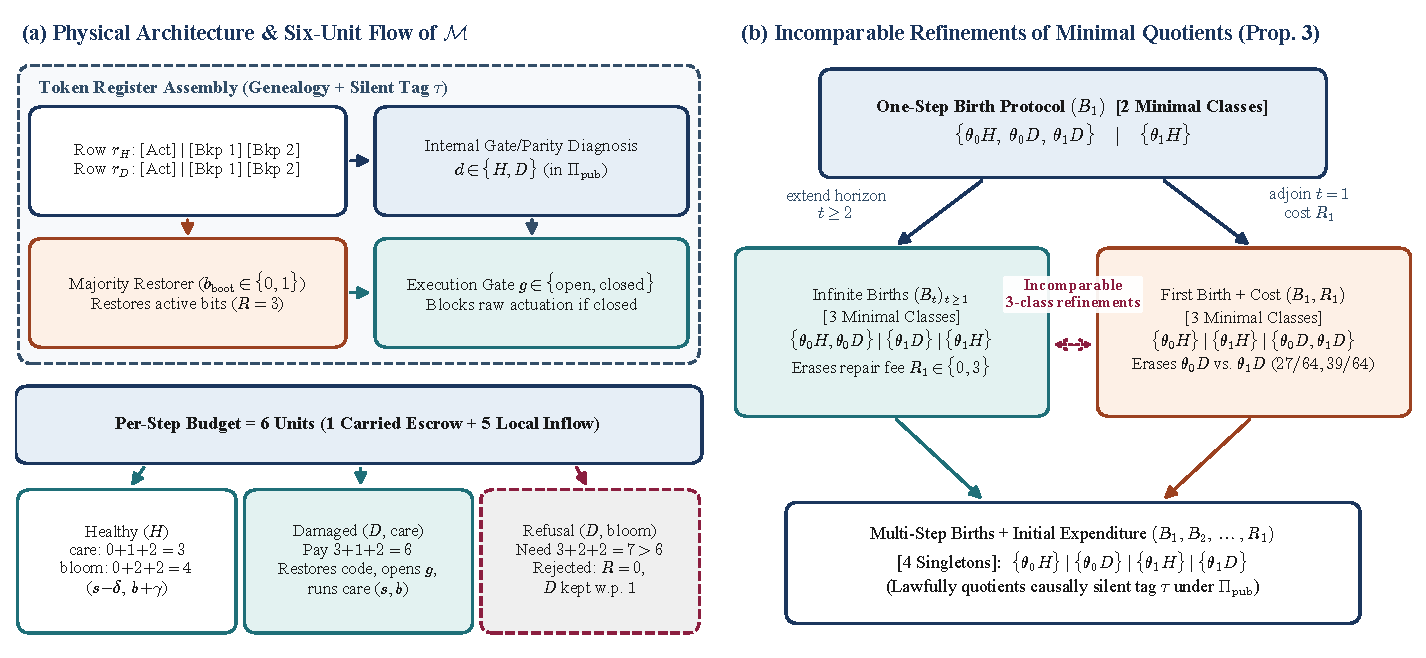
\includegraphics[width=0.98\linewidth,height=\textheight,keepaspectratio,alt={Register
architecture and predictive quotient lattice of \textbackslash
mathcal\{M\}. (a) Three-cell rows, diagnostic d, majority restorer, gate
g, and six-unit flow. (b) Diamond lattice of minimal protocol-law
partitions at fixed parameters (Proposition
3).}]{figures/fig1_architecture_and_lattice.pdf}
\caption{Register architecture and predictive quotient lattice of
\(\mathcal{M}\). (a) Three-cell rows, diagnostic \(d\), majority
restorer, gate \(g\), and six-unit flow. (b) Diamond lattice of minimal
protocol-law partitions at fixed parameters (Proposition 3).}
\end{figure}

\subsection{Lawful tag quotients versus von Neumann's
syntactic--constructor
gap}\label{lawful-tag-quotients-versus-von-neumanns-syntacticconstructor-gap}

\textbf{Proposition 4 (Silent-tag lumpability versus decoded-sequence
gate separation).} \emph{(a) Erasing silent tag \(\tau\) defines a
strong Markov lumpability \citep{burkeRosenblatt1958} commuting with
transitions, six-unit budgets, repair costs, genealogy, and expectations
across all \(\tau\)-blind policies lifted from the quotient (in
particular, across \(\Pi_{\mathrm{pub}}\)). (b) Projecting onto
majority-decoded code \(\theta \in \{\theta_0, \theta_1\}\) (even with
intact row parity) while erasing physical gate
\(g \in \{\mathrm{open}, \mathrm{closed}\}\) fails to determine raw
actuation: two intact \(\theta_1\) assemblies execute \texttt{bloom}
when \(g=\mathrm{open}\) (\(b+\gamma\)) but block raw actuation when
\(g=\mathrm{closed}\).}

Proposition 4 realizes von Neumann's \citeyearpar{vonNeumann1966}
separation between passive syntactic tape and active gated constructor
\citep{rosen1991, deacon2011}, qualitatively motivated in biology by
\emph{Escherichia coli} methyl-directed mismatch repair, where
hemimethylated \texttt{GATC} strands guide ATP-dependent
\texttt{MutS–MutL–MutH} initiation at replication forks
\citep{auWelshModrich1992, hasanLeach2015} (Section 6.2).

\section{Persistence, paid repair, and diachronic
bearers}\label{persistence-paid-repair-and-diachronic-bearers}

\subsection{Dynamical stability, servocontrol, paid repair, and
reciprocal
closure}\label{dynamical-stability-servocontrol-paid-repair-and-reciprocal-closure}

Universal loop or density signatures \citep{friston2013} conflate four
regimes (Table 3). First, \emph{passive invariance} (\(\dot{x} = -x\) on
contractible \(\mathbb{R}^n\), \(H_1(\mathbb{R}^n) = 0\)) yields compact
\(\omega(x_0) = \{0\}\) without cycles or repair. Second, \emph{external
servocontrol} \citep{rosenblueth1943, conantAshby1970} regulates targets
via fixed hardware it never rebuilds. Third, \emph{paid repair and
constraint closure}
\citetext{\citealp[§§64--65]{kant1790}; \citealp{varela1974}; \citealp{maturanaVarela1980}; \citealp{weberVarela2002}; \citealp{rosen1991}; \citealp{kauffman1993}; \citealp{deacon2011}; \citealp{mossio2009}; \citealp{montevilMossio2015}}
expend work to regenerate degrading constraints
\citep{jonas1966, thompson2007}: in \(\mathcal{M}\), active rows and
\(g\) degrade at rate \(q\) on \(\tau_{\mathrm{step}}=1\) and are
rebuilt via backups and \(b_{\mathrm{boot}}=1\) fixed on
\(\tau_{\mathrm{boot}} \gg 1\), whereas full Montévil--Mossio closure
adds a slow loop regenerating \(b_{\mathrm{boot}}\) and backups. Fourth,
\emph{adaptive viability}
\citep{aubinCellina1984, diPaolo2005, barandiaran2009, bich2024}
modulates modes near viability boundaries.

\Needspace{24\baselineskip}

{\def\LTcaptype{none} % do not increment counter
\begin{longtable}[]{@{}
  >{\raggedright\arraybackslash}p{(\linewidth - 6\tabcolsep) * \real{0.2500}}
  >{\raggedright\arraybackslash}p{(\linewidth - 6\tabcolsep) * \real{0.2500}}
  >{\raggedright\arraybackslash}p{(\linewidth - 6\tabcolsep) * \real{0.2500}}
  >{\raggedright\arraybackslash}p{(\linewidth - 6\tabcolsep) * \real{0.2500}}@{}}
\toprule\noalign{}
\begin{minipage}[b]{\linewidth}\raggedright
Persistence Regime
\end{minipage} & \begin{minipage}[b]{\linewidth}\raggedright
Sustaining Mechanism
\end{minipage} & \begin{minipage}[b]{\linewidth}\raggedright
Counterfactual Cut Signature
\end{minipage} & \begin{minipage}[b]{\linewidth}\raggedright
Paradigm Literature
\end{minipage} \\
\midrule\noalign{}
\endhead
\bottomrule\noalign{}
\endlastfoot
1. Passive invariance & Dissipative or conservative law (\(\dot{x}=-x\))
& Shifts orbit; zero constraint restoration & Topological dynamics \\
2. External servocontrol & Fixed feedback sensor--actuator & Regulates
state; zero hardware self-repair & \citet{rosenblueth1943};
\citet{conantAshby1970} \\
3a. Paid repair (\(\mathcal{M}\)) & Work restores \(g\), active code via
scaffolded \(b_{\mathrm{boot}}=1\) & Survives fast damage; halts if
\(b_{\mathrm{boot}}\) cut & \citet{vonNeumann1966};
\citet{auWelshModrich1992} \\
3b. Reciprocal closure & Slow loop on \(\tau_{\mathrm{boot}}\) also
regenerates \(b_{\mathrm{boot}}\) & Cutting slow loop degrades
\(b_{\mathrm{boot}}\) & \citet{kant1790}; \citet{varela1974};
\citet{rosen1991}; \citet{montevilMossio2015} \\
4. Adaptive viability & History-sensitive policy in kernel \(K^\star\) &
Separates finite memory \(m\ge 1\) from \(m=0\) &
\citet{aubinCellina1984}; \citet{diPaolo2005}; \citet{bich2024} \\
\end{longtable}
}

Table 3. Distinct regimes of temporal persistence, separating paid
endogenous repair (3a) from reciprocal closure (3b).

\subsection{Minimal cut-sets, finite-memory viability, and fixed-sample
limits}\label{minimal-cut-sets-finite-memory-viability-and-fixed-sample-limits}

Under monotone deletion failure on a downward-closed finite repertoire
\(\mathcal{I}\), destructive perturbations are uniquely represented by
the antichain of minimal cut-sets
\(\mathcal{V}_{\min}(\mathcal{C}, \mathcal{I})\) (\textbf{Proposition
5}, Appendix A.2)---isolating in \(\mathcal{M}\) bootstrap severance
(\(b_{\mathrm{boot}}=0\)), underfunding (\(2 < 3\)), and full three-cell
erasure \citep{coverThomas2006}, while failing under disinhibition.
Moreover (\textbf{Proposition 6}, Appendix A.2): \emph{(a)} on a
five-state system with maximal viable kernel
\(K^\star = \operatorname{gfp}(F_S) = S\) under pooled observation
\(h\), \emph{every} memoryless policy
\(\pi_0: \mathcal{O} \to \Delta(\mathcal{A})\) exits \(S\) in two steps
w.p. \(1/2\) whereas one-step memory
\(\pi_1: \mathcal{O}^2 \to \mathcal{A}\) maintains
\(\mathbb{P}_{\pi_1}(X_t \in K^\star\ \forall t \ge 0) = 1\) (Figure 2a)
\citep{kaelbling1998, papadimitriouTsitsiklis1987, sethTsakiris2018};
and \emph{(b)} for
\(Z_i \stackrel{\mathrm{i.i.d.}}{\sim} \mathrm{Bernoulli}(r)\), bounding
\(\mathbb{E}_r[\psi(Z_{1:n})] \le \alpha\) across all \(r \in (0,1]\)
forces \(\mathbb{E}_0[\psi] \le \alpha\) \citep{leCam1973, mayo2018}.

\subsection{Symmetrical fission as a stress test of relational
objecthood}\label{symmetrical-fission-as-a-stress-test-of-relational-objecthood}

Organisms persist through turnover while individuality splinters across
physiological, immunological, and Darwinian criteria
\citep{whitehead1929, clarke2010, godfreySmith2009, pradeu2012, maynardSmithSzathmary1995, dupreNicholson2018}.
Process \(\mathcal{M}\) separates parental retention from strict birth
despite identical post-step predictive classes \citep{wiggins2001}.
Symmetrical fission into equally continuous, intervention-stable,
cost-accountable daughters \(y_1 \neq y_2\) \citep{parfit1984}
stress-tests Criteria (1)--(3): \emph{both} satisfy all three equally,
yet transitivity blocks numerical identity with both, leaving parent
indexing (as in \(\mathcal{M}\)), clonal termination, versus lineage
tracking to explicit bearer conventions. Likewise, an absorbing chain's
\emph{quasi-stationary distribution} \(\nu_{\mathrm{QSD}}\) differs from
its \emph{Doob \(h\)-transformed} survivor law
\(\varpi(x) \propto \nu_{\mathrm{QSD}}(x)h(x)\)
\citep{doob1957, darrochSeneta1965, collet2013, cuciniello2026}.

\section{Optimization, bearer divergence, and the grounds of
purpose}\label{optimization-bearer-divergence-and-the-grounds-of-purpose}

\subsection{Evaluative underdetermination: reward shaping, gauge, and
bottleneck
rank}\label{evaluative-underdetermination-reward-shaping-gauge-and-bottleneck-rank}

Behavioral optimality never suffices for purpose: in inverse
reinforcement learning, policies fit an infinite reward cone
\citep[§3.1]{ngRussell2000}; in discounted or proper-absorbing episodic
dynamic programming \citep{blackwell1965, puterman1994}, potential
shaping \(r'(x,a,x') = r(x,a,x') + \beta\psi(x') - \psi(x)\) preserves
optimal policies \citep{ngHaradaRussell1999}; non-total preorders lack
scalar utilities \citep{krantz1971}; and resource--information scores
\(J = R - \lambda I\)---comparable to expected free energy
\citep{parrPezzuloFriston2022} and distinct from Tononi's
\citeyearpar{tononi2004} \(\Phi^{\mathrm{IIT}}\)---admit affine gauge
freedom \(R' = R + \lambda\chi\), \(I' = I + \chi\). Moreover
(\textbf{Proposition 7}, Appendix A.2), under healthy \(\theta_0\),
\(\Psi(s,b,q) := (s, b, bq)\) has \(\det D\Psi = b > 0\), ruling out
\emph{losslessly reconstructing \((s,b,bq)\) through any smooth
two-variable \((R,I)\) bottleneck}.

\subsection{Full-policy growth ceiling versus autonomous hereditary
attainment}\label{full-policy-growth-ceiling-versus-autonomous-hereditary-attainment}

With per-token six-unit sites, one-step output means are \(k_c = s+b\)
and \(k_b = s-\delta+b+\gamma\), giving \(\lambda_0 = k_c\) and
\(\lambda_1 = (1-q)k_b + q k_c\). Admissible policies
\(\pi \in \Pi_{\mathrm{pub}}\) read public history \(\mathcal{F}_t\)
(living counts, diagnoses \(d_u \in \{H, D\}\), genealogy, and past
receipts---including \(\pi_{\mathrm{dorm}}\), playing \texttt{care} on
\(H\) and \texttt{bloom} on \(D\)) with arbitrary joint randomization
across living tokens, blind to \(\tau\) and contemporaneous/future
noise.

\textbf{Theorem 1 (Full-policy growth ceiling versus autonomous
hereditary attainment).} \emph{For any strict parameters in Table 1 and
finite non-empty initial population \(P_0\), let
\(\rho_* := \max\{1, \lambda_0, \lambda_1\}\). (1) Across \textbf{all}
policies \(\pi \in \Pi_{\mathrm{pub}}\), there exists \(C > 0\) such
that \(\mathbb{E}_\pi[N_t] \le C \rho_*^t\) for all \(t \ge 0\), and a
stationary policy in \(\Pi_{\mathrm{pub}}\) attains
\(\Theta(\rho_*^t)\). (2) Under \textbf{autonomous multi-generational
execution of the fixed hereditary program \(\theta_i\)}
(\(i \in \{0,1\}\)) from a single damaged founder \(\theta_i D\), paid
first-step repair (\(R_1=3\)), gate-mediated execution, and
\(\Theta(\rho_*^t)\) attainment hold jointly iff
\((\gamma \le \delta \land k_c \ge 1)\) for \(\theta_0\), and iff
\((\gamma \ge \delta \land \lambda_1 \ge 1)\) for \(\theta_1\).}

Separating the two quantifiers in Theorem 1 is essential: if a
controller in \(\Pi_{\mathrm{pub}}\) may \emph{abandon} hereditary
execution after \(t=1\), paid repair and \(\Theta(\rho_*^t)\) attainment
hold even in the subcritical regime. At
\((s,\delta,b,\gamma,q) = (1/2, 1/4, 1/4, 1/8, 1/3)\), \(k_c = 3/4\),
\(k_b = 5/8\), \(\lambda_1 = 2/3\), and \(\rho_* = 1\): neither
autonomous \(\theta_0\) nor autonomous \(\theta_1\) attains
\(\rho_*=1\), yet running \texttt{care} at \(t=1\) (\(R_1=3\), reopening
\(g\)) and switching to \(\pi_{\mathrm{dorm}}\) for \(t \ge 2\) retains
a damaged parent at \(t=2\) w.p. \(sq = 1/6\) (and leaves at least one
\(D\)-token w.p. \(17/72\)), yielding \(\Theta(1)\) via arrested
dormancy rather than active lineage reproduction.

Theorem 1 (Figure 2b) yields three further separations. First, in
subcritical Regime I
(\(\bar{\lambda} := \max\{\lambda_0,\lambda_1\} < 1\)), \(\rho_* = 1\)
arises from rejected damaged \texttt{bloom}---analogous to dormant
persisters---yet expected potential drops by at least
\((1-\bar{\lambda})k_c > 0\) per actively executed step, forcing finite
cumulative expected births
\(\mathbb{E}_\pi[\sum_{t\ge 1} B_t] \le (b+\gamma)V(P_0)/[(1-\bar{\lambda})k_c] < \infty\)
for \emph{every} \(\pi \in \Pi_{\mathrm{pub}}\): attaining \(\rho_*=1\)
here preserves only frozen tokens rather than active organization or
ongoing reproduction, so any claim of ``good maintenance'' must specify
its bearer and criterion first. Second, in Regime III
(\(\gamma > \delta, \lambda_1 \ge 1\)), autonomous \texttt{bloom}
maximizes lineage growth while \emph{reducing} parent survival
(\(s-\delta < s\)), splitting organismal persistence from lineage
multiplication \citep{okasha2006, godfreySmith2009} and
\emph{differential retention} from \emph{differential reproduction}
\citep{garson2019}. Third, at critical \((2/3, 1/8, 1/4, 1/4, 1/3)\),
\(\lambda_1 = \rho_* = 1\) yet
\(\mathbb{E}_{\theta_1 D}[N_t] = 11/12 < 1\) for all \(t \ge 1\)
(\(k_c=11/12, k_b=25/24\)). At supercritical
\((3/4, 1/8, 3/8, 1/4, 1/3)\), independent founders \(\theta_1 H\) and
\(\theta_0 H\) satisfy
\(\mathbb{P}(N_1^{(1)} = 0 \land N_1^{(0)} > 0) = 243/2048\) (early
\(\theta_1\) extinction while \(\theta_0\) survives); for share
\(S_1 := N_1^{(1)}/(N_1^{(1)} + N_1^{(0)})\) (\(0\) on joint
extinction), \(\mathbb{E}[S_1] = 2095/4096\),
\(\mathbb{E}[S_1 \mid N_1^{(1)} + N_1^{(0)} > 0] = 2095/4006\), and
\(\mathbb{E}[N_1^{(1)}]/\mathbb{E}[N_1^{(1)}+N_1^{(0)}] = 10/19\)
\citep{price1970, athreyaNey1972}.

\begin{figure}
\centering
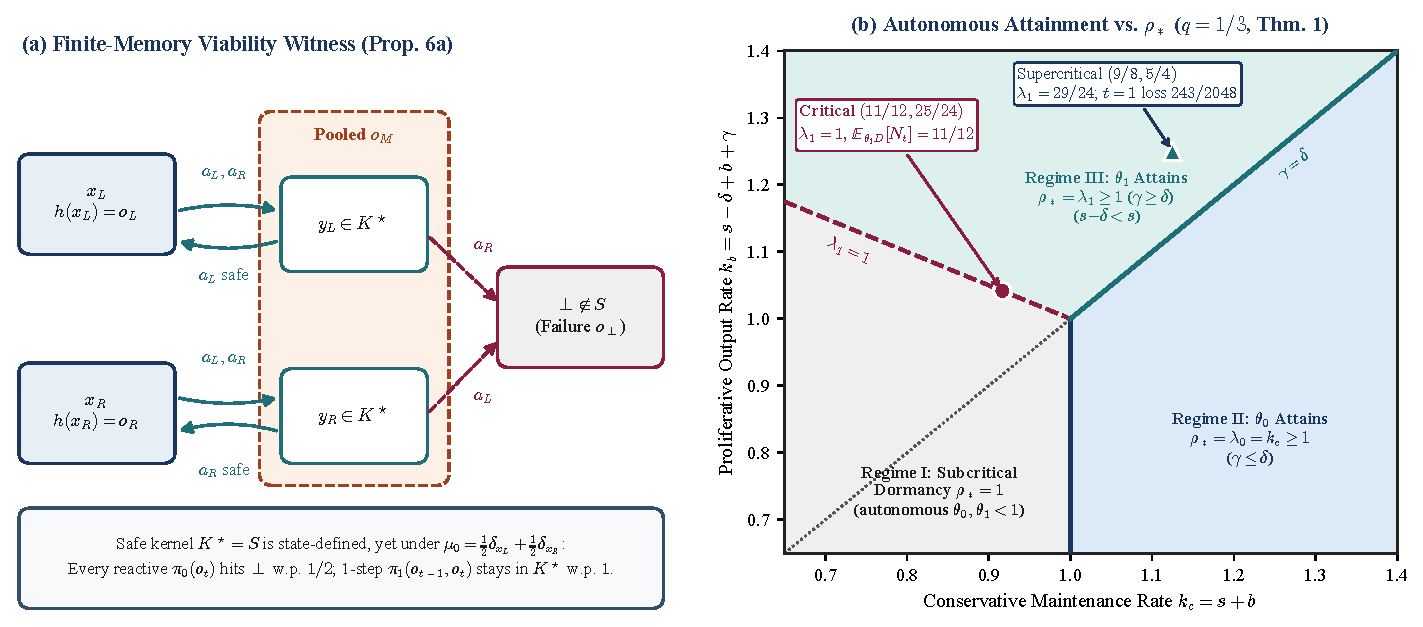
\includegraphics[width=0.98\linewidth,height=\textheight,keepaspectratio,alt={Finite-memory
viability and demographic phase diagram. (a) Five-state viability
witness (Proposition 6a): reactive \textbackslash pi\_0(o\_t) fails in
two steps w.p. 1/2, while one-step memory \textbackslash
pi\_1(o\_\{t-1\},o\_t) stays in K\^{}\textbackslash star w.p. 1. (b)
Exact (k\_c, k\_b) phase diagram at q = 1/3 (Theorem 1), marking
dormancy (\textbackslash rho\_*=1), \textbackslash theta\_0 and
\textbackslash theta\_1 attainment, and witnesses (11/12, 25/24) and
(9/8, 5/4).}]{figures/fig2_memory_and_phase.pdf}
\caption{Finite-memory viability and demographic phase diagram. (a)
Five-state viability witness (Proposition 6a): reactive \(\pi_0(o_t)\)
fails in two steps w.p. \(1/2\), while one-step memory
\(\pi_1(o_{t-1},o_t)\) stays in \(K^\star\) w.p. \(1\). (b) Exact
\((k_c, k_b)\) phase diagram at \(q = 1/3\) (Theorem 1), marking
dormancy (\(\rho_*=1\)), \(\theta_0\) and \(\theta_1\) attainment, and
witnesses \((11/12, 25/24)\) and \((9/8, 5/4)\).}
\end{figure}

\subsection{Four stratified grounds of purpose and the normativity
challenge}\label{four-stratified-grounds-of-purpose-and-the-normativity-challenge}

Causal-role analysis \citep{cummins1975} lacks malfunction norms
\citep{davies2001}, selected-effects etiology
\citep{wright1973, millikan1984, neander1991, godfreySmith1994} misses
de novo regulation, and organizational accounts
\citep{mossio2009, bich2024} face Corti's \citeyearpar[§3]{corti2023}
and Bedau's \citeyearpar{bedau1992} challenge: why does existential
dependence support a functional \emph{ought}? Table 4 and Figure 3
stratify four non-interchangeable grounds:

\Needspace{24\baselineskip}

{\def\LTcaptype{none} % do not increment counter
\begin{longtable}[]{@{}
  >{\raggedright\arraybackslash}p{(\linewidth - 6\tabcolsep) * \real{0.2500}}
  >{\raggedright\arraybackslash}p{(\linewidth - 6\tabcolsep) * \real{0.2500}}
  >{\raggedright\arraybackslash}p{(\linewidth - 6\tabcolsep) * \real{0.2500}}
  >{\raggedright\arraybackslash}p{(\linewidth - 6\tabcolsep) * \real{0.2500}}@{}}
\toprule\noalign{}
\begin{minipage}[b]{\linewidth}\raggedright
Rung
\end{minipage} & \begin{minipage}[b]{\linewidth}\raggedright
Ground of Attribution
\end{minipage} & \begin{minipage}[b]{\linewidth}\raggedright
Bearer \& Required Evidence
\end{minipage} & \begin{minipage}[b]{\linewidth}\raggedright
Normative Scope \& Limit
\end{minipage} \\
\midrule\noalign{}
\endhead
\bottomrule\noalign{}
\endlastfoot
\textbf{1. Systemic role} & Constitutive decomposition
\citep{cummins1975, craver2007} & Part in capacity \(\Psi\); ablation
test & Explanatory relevance; \textbf{no} malfunction norm
\citep{davies2001} \\
\textbf{2. Regulatory repair} & Paid repair + control
\citep{nagel1977, mossio2009, diPaolo2005, bich2024} & Organism token;
gate/repair into \(K^\star\) & \emph{System-conditional functional
standard}; \textbf{not} categorical value \\
\textbf{3. Selective history} & Differential retention/reproduction
\citep{wright1973, millikan1984, garson2019} & Selected
lineage/repertoire; ancestral selection & \emph{Retrospective proper
function}; can \textbf{conflict} with Rung 2 \\
\textbf{4. Practical reason} & Reflective justification
\citep{korsgaard1996, scanlon1998, list2019} & Deliberative agent;
normative scrutiny & \emph{Justificatory ought}; \textbf{never} entailed
by Rungs 1--3 \citep{street2006} \\
\end{longtable}
}

Table 4. Four stratified grounds of functional and purposive
explanation.

\begin{enumerate}
\def\labelenumi{\arabic{enumi}.}
\tightlist
\item
  \textbf{Operational conditional standards at Rung 2---and where
  Corti's objection retains force.} Pointing out that biology lacks
  moral obligations misses \citet{corti2023}; instead, Rung 2 supplies
  an \emph{operational, system-conditional standard}
  \citep{nagel1977, walsh2015} while pinpointing where Corti's challenge
  retains force \citep{bedau1992, cuciniello2026}. \emph{Given}
  executable integrity in \(K^\star\), \(\mathcal{M}\) separates
  \emph{(i) malfunction} (\(b_{\mathrm{boot}}=0\) or stuck
  \(g=\mathrm{closed}\)), \emph{(ii) accidental side-effect survival}
  (rejected \texttt{bloom}), and \emph{(iii) costly normal operation}
  (damaged \texttt{care}, \(R_1=3\)). Yet answering
  \citet{corti2023}---what bridges causal dependence to an intrinsic
  functional \emph{ought}---is settled automatically by neither
  slow-timescale reciprocal closure \citep{montevilMossio2015} nor Rung
  3 selection \citep{millikan1984, garson2019}: they remain distinct
  candidate grounds that each require independent defense (why
  persistence of \emph{this} closed regime is normative rather than mere
  stability; how ancestral selection binds \emph{this} present token),
  reinforcing Rung 2's system-conditional scope.
\item
  \textbf{Prospective demographic advantage versus retrospective Rung 3
  function.} In a preset environment with \(\gamma > \delta\),
  \texttt{bloom} impairs Rung 2 parent survival (\(s-\delta < s\)) while
  raising \emph{prospective} lineage multiplication
  (\(\lambda_1 > \lambda_0\)). Respecting Table 4's evidential standard,
  \(\lambda_1 > \lambda_0\) alone is demographic propensity, \emph{not}
  yet a Rung 3 proper function: Rung 3 attribution additionally requires
  historical cohort-selection evidence that \(\theta_1\) persisted or
  spread \emph{because} of that proliferative effect.
\item
  \textbf{Scope of Rung 4.} Process \(\mathcal{M}\) contains no Rung 4
  witness; Rung 4 marks the boundary showing that Rungs 1--3 never by
  themselves entail practical endorsement
  \citep{korsgaard1996, street2006, list2019}.
\end{enumerate}

\begin{figure}
\centering
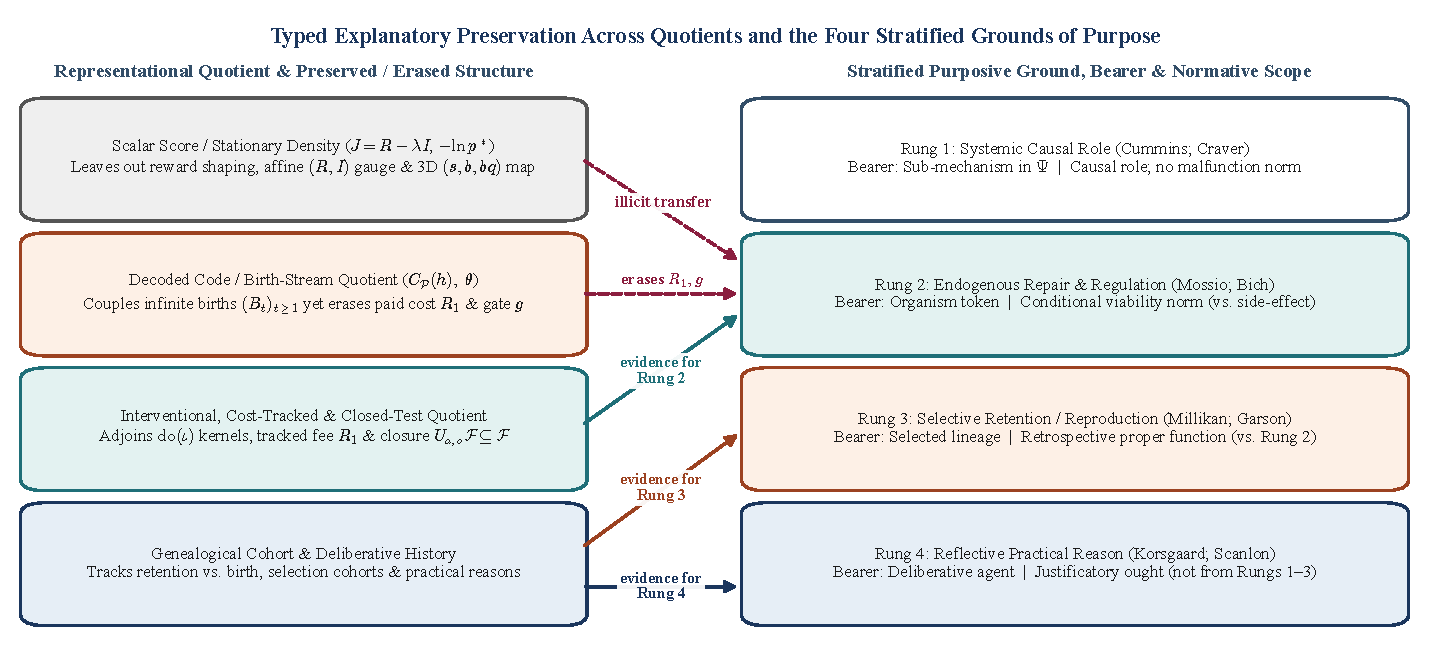
\includegraphics[width=0.98\linewidth,height=\textheight,keepaspectratio,alt={Typed
explanatory preservation across quotients (left) aligned with the four
stratified grounds of purposive attribution and required evidence
channels (right).}]{figures/fig3_preservation_and_rungs.pdf}
\caption{Typed explanatory preservation across quotients (left) aligned
with the four stratified grounds of purposive attribution and required
evidence channels (right).}
\end{figure}

\section{Competitor diagnostics, objections, and empirical
tests}\label{competitor-diagnostics-objections-and-empirical-tests}

\subsection{Diagnosing cross-protocol leaps in contemporary
programs}\label{diagnosing-cross-protocol-leaps-in-contemporary-programs}

\emph{(1) Active inference:} inside each token, \((r_H, r_D)\)
influences births only along \((r_H, r_D) \to (d_t, g_t, a_t) \to B_t\)
through diagnostic \(d_t\), gate \(g_t\), \emph{and} executed action
\(a_t\) (omitting \(a_t\) fails local mediation since \(\theta_0 H\) and
\(\theta_1 H\) share \(d_1=H, g_1=\mathrm{open}\) yet induce birth rates
\(b\) vs.~\(b+\gamma\)). Such local mediation does not establish
Friston's stationary nonequilibrium conditional-independence blanket
assumptions
\citep{friston2013, parrPezzuloFriston2022, bruineberg2022, raja2021};
our distinct cross-protocol result is that \emph{even an output
interface sufficient to predict the entire birth stream
\((B_t)_{t\ge 1}\) can erase paid repair \(R_1\) (\(3\) vs.~\(0\))},
while composite scores retain affine gauge freedom \citep{biehl2021} and
parent survival diverges from lineage growth, requiring Rung 2 hardware
anchors \citep{sethTsakiris2018}. \emph{(2) Computational mechanics:}
minimal \(\varepsilon\)-transducers
\citep{shaliziCrutchfield2001, barnettCrutchfield2015} and
macro-emergence \citep{hoel2013} are protocol-relative; Proposition 3
maps their transfer boundary. \emph{(3) Organizational vs.~evolutionary
teleology:} gate \(g\) captures state-sensitive modulation
\citep{bich2024} while genealogical records govern the handoff from Rung
2 tokens to Rung 3 cohorts \citep{cuciniello2026}.

\subsection{Constructive unification and replies to four
objections}\label{constructive-unification-and-replies-to-four-objections}

Separate models \(\exists x\,R(x)\) and \(\exists y\,O(y)\) do not
entail \(\exists z\,[R(z)\land O(z)]\) when repair consumes half the
six-unit budget (\(3/6\)) and blocks damaged \texttt{bloom}
\citep{friedman1974, kitcher1989}; Theorem 1 establishes exact
constrained compatibility.

\begin{enumerate}
\def\labelenumi{\arabic{enumi}.}
\tightlist
\item
  \emph{Constructive empiricism suffices \citep{vanFraassen1980}.}
  Formal theorems never compel realism; our case is comparative
  \citep{hacking1983, woodward2003}. From damaged conservative founder
  \((\theta_0, D)\) (\(r_H, r_D\) active bits flipped,
  \(g=\mathrm{closed}\)), specify two competing mechanisms under the
  six-unit budget (\(3+1+2=6\)): \(\mathcal{M}_{\mathrm{vote}}\)
  majority-votes via \(b_{\mathrm{boot}}\), whereas
  \(\mathcal{M}_{\mathrm{bypass}}\) uses a hardwired auxiliary
  \texttt{care}-latch not reading \(b_{\mathrm{boot}}\). Under
  \(b_{\mathrm{boot}}=1\), on \((D,\mathrm{care})\) both pay \(R_t=3\),
  restore \((r_H,r_D)\) and \(g \leftarrow \mathrm{open}\) at step end,
  and transition into the exact same post-step law
  \((I_{\mathrm{ret}}, B_t) \sim \mathrm{Bern}(s)\otimes\mathrm{Bern}(b)\)
  of \(\theta_0\)-tokens (damaged w.p. \(q\), re-engaging whenever \(D\)
  recurs), inducing \emph{identical} joint laws on
  \(((B_t,R_t))_{t\ge 1}\). Under \(\mathrm{do}(b_{\mathrm{boot}}=0)\),
  \(\mathcal{M}_{\mathrm{vote}}\) fails voting
  (\(g=\mathrm{closed}, R_t=0\), recovery probability \(0\),
  \(\mathbb{E}[B_1\mid \mathrm{do}(b_{\mathrm{boot}}=0)]=0\),
  \(B_t=0\ \forall t\ge 1\)), whereas \(\mathcal{M}_{\mathrm{bypass}}\)
  recovers w.p. \(1\) (\(R_1=3\),
  \(\mathbb{E}[B_1\mid \mathrm{do}(b_{\mathrm{boot}}=0)]=b>0\);
  \citet{rubenstein2017}; Online Supplement), yielding differential
  severe-testing support \citep{mayo2018}.
\item
  \emph{Preservation is trivially analytic.} Fiber factorization
  (\(F = \bar{F}\circ q\)) is analytic once \(F\) and \(q\) are fixed;
  the substantive work is proving \emph{which} compressions destroy
  \emph{which} invariants---including fixed-parameter two-step birth
  saturation alongside cost erasure (Proposition 3),
  sequence-versus-gate separation (Proposition 4b), finite-memory
  viability (Proposition 6a), and critical deficits (\(11/12 < 1\)).
\item
  \emph{Stipulated scaffolding falls short of full closure.} Exogenous
  energy inflow is shared by living cells and does not render repair
  fictitious \citep{jonas1966, montevilMossio2015}. Because
  \(b_{\mathrm{boot}}=1\) is fixed on the modeled horizon,
  \(\mathcal{M}\) establishes fast-timescale paid repair (Table 3, 3a),
  leaving slow regeneration of \(b_{\mathrm{boot}}\) (3b) and Rung 3
  selection explicit.
\item
  \emph{Empirical discrimination between rival mechanisms.} Mapping
  variables onto interventions \citep{craver2007, rubenstein2017} on an
  \emph{engineered fault-tolerant register} initialized at
  \((\theta_0, D)\) tests cost-free pass-through \emph{(H0)}
  (\(R_1=0\)), majority-vote repair
  \emph{(\(\mathcal{M}_{\mathrm{vote}}\))}, and auxiliary-latch bypass
  \emph{(\(\mathcal{M}_{\mathrm{bypass}}\))} across: \emph{(Arm 1)}
  matched \((B_t)_{t\ge 1}\) laws under \(b_{\mathrm{boot}}=1\);
  \emph{(Arm 2)} per-cycle repair-energy metering (\(R_1=0\) vs.~\(3\));
  \emph{(Arm 3)} \(\mathrm{do}(b_{\mathrm{boot}}=0)\) versus gate clamp
  \(\mathrm{do}(g=\mathrm{closed})\) at intact \(\theta_0\), separating
  \(\mathcal{M}_{\mathrm{vote}}\) (\(B_1=0\)) from
  \(\mathcal{M}_{\mathrm{bypass}}\) (\(\mathbb{E}[B_1]=b>0\)); and
  \emph{(Arm 4)} six-unit inflow titration tracking parent retention
  versus child spawning \citep{mayo2018}. In biology, \emph{E. coli}
  \texttt{MutS–MutL–MutH} repair versus translesion bypass
  \citep{auWelshModrich1992, hasanLeach2015} provides qualitative
  motivation, though bulk cellular ATP pools confound multiple pathways
  and cannot alone isolate \(R_1\).
\end{enumerate}

\section{Conclusion}\label{conclusion}

When two rival explanations share the exact same predictive law on an
output channel, what additional evidence warrants accepting one over the
other? Our results show that extending observations along different
coordinates produces mutually incomparable refinements, that autonomous
hereditary attainment of full-policy growth ceilings separates sharply
from plastic dormancy switching, and that parent survival can oppose
lineage multiplication. Calibrating relational objecthood and four-rung
bearer-indexed purpose strictly to these evidential boundaries preserves
explanatory unity without overclaiming beyond what mechanism, repair
budgets, and selection history warrant.

\appendix

\section{Self-contained proofs of Propositions 1--7 and Theorem
1}\label{self-contained-proofs-of-propositions-17-and-theorem-1}

\emph{Proof of Proposition 1.} Each countably generated
\(\Sigma_{\mathcal{Y}_i}\) is generated by a countable \(\pi\)-system
\(\mathcal{G}_i = \{G_{i,m}\}_{m\in\mathbb{N}}\) with
\(\mathcal{Y}_i \in \mathcal{G}_i\) \citep{kallenberg2021}. By
sufficiency of \(q\), for each \(i \in \mathcal{I}\) there exists
\(\widetilde{K}_i\) such that
\(N_i := \bigcup_{m\in\mathbb{N}} \{h \in \mathcal{H} : K_i(h, G_{i,m}) \neq \widetilde{K}_i(q(h), G_{i,m})\} \in \Sigma_{\mathcal{H}}\)
satisfies \(\mu(N_i) = 0\); by Dynkin's \(\pi\)-\(\lambda\) theorem,
\(K_i(h, \cdot) = \widetilde{K}_i(q(h), \cdot)\) for all
\(h \notin N_i\). Defining
\(\psi(z) := (\widetilde{K}_i(z, \cdot))_{i\in\mathcal{I}}\) and
\(N := \bigcup_{i\in\mathcal{I}} N_i\), countability of \(\mathcal{I}\)
gives \(\mu(N) \le \sum_{i\in\mathcal{I}} \mu(N_i) = 0\), with
\(C_{\mathcal{P}}(h) = \psi(q(h))\) on \(\mathcal{H}\setminus N\).
\(\square\)

\emph{Proof of Proposition 2.} Let
\(b'_{a,o}(x') = \sum_{x} b(x) T(x'\mid x,a) O(o\mid a,x')\); then
\(\langle b'_{a,o}, f\rangle = \langle b, U_{a,o}f\rangle\) and
\(p(o\mid b,a) = \langle b, U_{a,o}\mathbf{1}\rangle\).
(\emph{Sufficiency}) If \(U_{a,o}\mathcal{F} \subseteq \mathcal{F}\) and
\(b \equiv_{\mathcal{F}} \tilde{b}\), then
\(U_{a,o}\mathbf{1} \in \mathcal{F}\) gives
\(p(o\mid b,a) = p(o\mid \tilde{b},a)\), and for \(p(o\mid b,a) > 0\),
\(\langle \mathrm{Bayes}(b,a,o), f\rangle = \langle b, U_{a,o}f\rangle / p(o\mid b,a) = \langle \mathrm{Bayes}(\tilde{b},a,o), f\rangle\)
(\(\forall f \in \mathcal{F}\)). (\emph{Necessity}) Assume (i)--(ii) on
\(\Delta(\mathcal{X})\). For \(v \in \mathcal{F}^\perp\),
\(\langle v, \mathbf{1}\rangle = 0\). Perturbing
\(b^\circ(x) = 1/|\mathcal{X}|\) to
\(\tilde{b} = b^\circ + \varepsilon v \in \Delta(\mathcal{X})\), (i)
forces \(\langle v, U_{a,o}\mathbf{1}\rangle = 0\)
(\(\forall v \in \mathcal{F}^\perp\)), so
\(U_{a,o}\mathbf{1} \in \mathcal{F}\). For \(f \in \mathcal{F}\), if
\(p_0 := p(o\mid b^\circ, a) = 0\), positivity of \(b^\circ\) gives
\(U_{a,o}\mathbf{1} \equiv 0\) and \(U_{a,o}f = 0 \in \mathcal{F}\); if
\(p_0 > 0\), (ii) gives \(\langle v, U_{a,o}f\rangle / p_0 = 0\)
(\(\forall v \in \mathcal{F}^\perp\)), so \(U_{a,o}f \in \mathcal{F}\).
\(\square\)

\emph{Proofs of Propositions 5, 6, and 7.} \emph{(Prop. 5)} Upward
closure follows from monotonicity; downward closure of finite
\(\mathcal{I}\) yields a minimum-cardinality \(M \subseteq D\) in
\(\mathcal{F}\), lying in the unique antichain \(\mathcal{V}_{\min}\).
\emph{(Prop. 6a)} On \(\mathcal{X} = \{x_L, x_R, y_L, y_R, \bot\}\),
\(S = \{x_L, x_R, y_L, y_R\}\), \(\mathcal{A} = \{a_L, a_R\}\), set
\(h(x_L)=o_L\), \(h(x_R)=o_R\), \(h(y_L)=h(y_R)=o_M\),
\(h(\bot)=o_\bot\), with \(x_L \to y_L\), \(x_R \to y_R\) under
\(\{a_L,a_R\}\); \(y_L \xrightarrow{a_L} x_L\),
\(y_L \xrightarrow{a_R} \bot\); \(y_R \xrightarrow{a_R} x_R\),
\(y_R \xrightarrow{a_L} \bot\); and \(\bot\) absorbing
(\(K^\star = S\)). Under
\(\mu_0 = \frac{1}{2}\delta_{x_L} + \frac{1}{2}\delta_{x_R}\), any
\(\pi_0(a_L \mid o_M) = p\) gives
\(\mathbb{P}_{\pi_0}(X_2 = \bot) = \frac{1}{2}(1-p) + \frac{1}{2}p = \frac{1}{2}\),
whereas \(\pi_1(o_L,o_M)=a_L\), \(\pi_1(o_R,o_M)=a_R\) keeps
\(X_t \in K^\star\) w.p. \(1\). \emph{(Prop. 6b)}
\(|g(0) - g(\varepsilon)| \le d_{\mathrm{TV}}(\mathrm{Bern}(0)^{\otimes n}, \mathrm{Bern}(\varepsilon)^{\otimes n}) = 1 - (1-\varepsilon)^n \le n\varepsilon\),
so \(\sup_{r>0} g(r) \le \alpha \implies g(0) \le \alpha\). \emph{(Prop.
7)}
\(\det D\Psi(s,b,q) = \det \bigl(\begin{smallmatrix}1&0&0\\0&1&0\\0&q&b\end{smallmatrix}\bigr) = b > 0\),
contradicting \(\operatorname{rank}(Dg \cdot Df) \le 2\). \(\square\)

\emph{Proofs of Propositions 3 and 4.} Across any fixed strict Table 1
vector (\(\gamma > 0\), \(s+b > 0\), \(1-q > 0\)): at \(t=1\),
\(\theta_0 H\) (\(R_1=0\)) and repaired \(\theta_0 D, \theta_1 D\)
(\(R_1=3\)) run \texttt{care} (\(B_1 \sim \mathrm{Bern}(b)\)), while
\(\theta_1 H\) (\(R_1=0\)) runs \texttt{bloom}
(\(B_1 \sim \mathrm{Bern}(b+\gamma)\)), giving two \(B_1\)-classes and
three \((B_1,R_1)\)-classes. After \(t=1\), \(\theta_0 H\) and
\(\theta_0 D\) leave identically distributed \(\theta_0\)-populations
\((I_{\mathrm{ret}}, B_1) \sim \mathrm{Bern}(s)\otimes\mathrm{Bern}(b)\)
damaged w.p. \(q\), coupling \((B_t)_{t\ge 1}\) identically. At \(t=2\),
\(\mathbb{E}[N_1] = s+b\) for \(\theta_0 D\) and \(\theta_1 D\), giving
\(\mathbb{E}_{\theta_0 D}[B_2] = (s+b)b\) versus
\(\mathbb{E}_{\theta_1 D}[B_2] = (s+b)[(1-q)(b+\gamma)+qb]\); their
difference \((s+b)(1-q)\gamma > 0\) yields three \((B_1,B_2)\)-classes
(\(27/64\) vs.~\(39/64\) at \((3/4,1/8,3/8,1/4,1/3)\)) and four
\((B_1,B_2,R_1)\)-singletons, with mutual Blackwell non-simulability
from \(\theta_0 H \sim_{(B_1,B_2)} \theta_0 D\) and
\(\theta_0 D \sim_{(B_1,R_1)} \theta_1 D\) (whereas from \(\theta_1 D\)
at \((3/4,3/8,1/4,1/3)\), \(\delta \in \{1/8,1/4\}\) share \((B_1,B_2)\)
laws since \(\delta\) enters only step-2 survival, splitting
\(\mathbb{E}[B_3] = k_c\lambda_1(\delta)(13/24)\) into \(377/512\)
vs.~\(351/512\)). For Prop. 4, \(\tau\) enters no kernel or cost rule,
commuting with \(\tau\)-blind policies, whereas intact \(\theta_1\)
assemblies diverge under \(g=\mathrm{open}\) vs.~\(\mathrm{closed}\).
\(\square\)

\emph{Proof of Theorem 1.} \textbf{(1)} Set \(v(H) := \max\{k_c, k_b\}\)
and \(v(D) := k_c\) (\(0 < k_c \le v(x) \le v_{\max}\)). Any executed
step with mean \(k \in \{k_c, k_b\}\) gives
\((L_a v)(x) = k[(1-q)v(H) + q v(D)]\). Whether \(\gamma \le \delta\)
(\(v \equiv k_c, \bar{\lambda} := \max\{\lambda_0,\lambda_1\} = k_c\))
or \(\gamma > \delta\)
(\(v(H)=k_b, v(D)=k_c, \bar{\lambda}=\lambda_1\)), every actively
executed step satisfies \((L_a v)(x) \le \bar{\lambda} v(x)\) while
rejected \((D,\mathrm{bloom})\) yields \(v(D) \le \rho_* v(D)\) and
\texttt{stop} yields \(0\). Summing \(V(P_t) = \sum_{u\in P_t} v(x_u)\)
under \(\pi \in \Pi_{\mathrm{pub}}\) gives
\(\mathbb{E}_\pi[V(P_{t+1})\mid \mathcal{F}_t] \le \rho_* V(P_t)\) and
\(\mathbb{E}_\pi[N_t] \le (v_{\max}|P_0|/k_c)\rho_*^t\); when
\(\bar{\lambda} < 1\), each active token drops expected \(V\) by
\(\ge (1-\bar{\lambda})k_c\), so telescoping bounds active steps and
yields
\(\mathbb{E}_\pi[\sum_{t\ge 1} B_t] \le (b+\gamma)V(P_0)/[(1-\bar{\lambda})k_c] < \infty\).
Tightness holds via \(\pi_{\mathrm{dorm}} \in \Pi_{\mathrm{pub}}\) when
\(\rho_*=1\)
(\(\mathbb{E}_{\pi_{\mathrm{dorm}}}[N_t] \ge \min\{1, sq\}\)),
stationary \(\theta_0\) when \(\rho_*=\lambda_0\), and stationary
\(\theta_1\) when \(\rho_*=\lambda_1\). \textbf{(2)} Under autonomous
execution from damaged founders,
\(\mathbb{E}_{\theta_0 D}[N_t] = k_c^t\)
(\(\Theta(\rho_*^t) \iff \gamma\le\delta \land k_c\ge 1\)) and
\(\mathbb{E}_{\theta_1 D}[N_t] = k_c \lambda_1^{t-1}\) for \(t \ge 1\)
(\(\Theta(\rho_*^t) \iff \gamma\ge\delta \land \lambda_1\ge 1\)). Under
switching in \(\Pi_{\mathrm{pub}}\) at \((1/2,1/4,1/4,1/8,1/3)\)
(\(k_c=3/4, k_b=5/8, \lambda_1=2/3, \rho_*=1\)), \texttt{care} at
\(t=1\) (\(R_1=3\)) then \(\pi_{\mathrm{dorm}}\) retains a \(D\)-parent
at \(t=2\) w.p. \(sq = 1/6\) (\(\ge 1\) \(D\)-token w.p. \(17/72\)),
giving \(\mathbb{E}[N_t] \ge 1/6\). At \((2/3,1/8,1/4,1/4,1/3)\),
\(k_c=11/12, k_b=25/24, \lambda_1=1\),
\(\mathbb{E}_{\theta_1 D}[N_t] = 11/12\). At \((3/4,1/8,3/8,1/4,1/3)\),
\(N_1^{(1)} \sim (9/64, 30/64, 25/64)\) and
\(N_1^{(0)} \sim (5/32, 18/32, 9/32)\), giving
\(\mathbb{P}(N_1^{(1)}=0 \land N_1^{(0)}>0) = \frac{243}{2048}\),
\(\mathbb{E}[N_1^{(1)}]/\mathbb{E}[N_1^{(1)}+N_1^{(0)}] = \frac{10}{19}\),
\(\mathbb{E}[S_1] = \frac{2095}{4096}\), and
\(\mathbb{E}[S_1 \mid N_1^{(1)}+N_1^{(0)} > 0] = \frac{2095}{4006}\).
\(\square\)

\section*{Declarations}\label{declarations}
\addcontentsline{toc}{section}{Declarations}

\textbf{Competing interests, code availability, and AI disclosure.} The
author(s) declare no competing interests or external funding. Anonymized
zero-dependency Python 3 scripts verifying all exact rational identities
and multi-step transitions (\texttt{verify\_standalone.py}, runnable via
\texttt{python3\ verify\_standalone.py}) and generating Figures 1--3
(\texttt{generate\_figures.py}) accompany this submission. The human
author(s) conceived the philosophical problem, core framework,
regenerative model, and proofs, directed all revisions, verified every
calculation and citation, and bear full academic responsibility; ChatGPT
6 Astra assisted with adversarial referee-style stress-testing and
formal/conceptual critique (reachable-set scope, fixed-parameter
saturation and three-step \(\delta\) witness, subcritical finite-birth
bound, and causal-abstraction specification), and Gemini 4 Carbon
implemented \texttt{fractions.Fraction} verification and Matplotlib
figure scripts, audited BibTeX/TeX builds, and assisted with prose
formatting.

\clearpage
\begingroup
\setstretch{1.02}
\small
\setlength{\bibsep}{5pt}
\bibliographystyle{plainnat}
\bibliography{references}
\endgroup
\end{document}
